% !TEX root = ../main.tex

\section{Communication Tools}
\begin{frame}{Telephone}
	\begin{columns}[T,onlytextwidth]
		\column{0.5\textwidth}
		\begin{figure} 
			\centering
			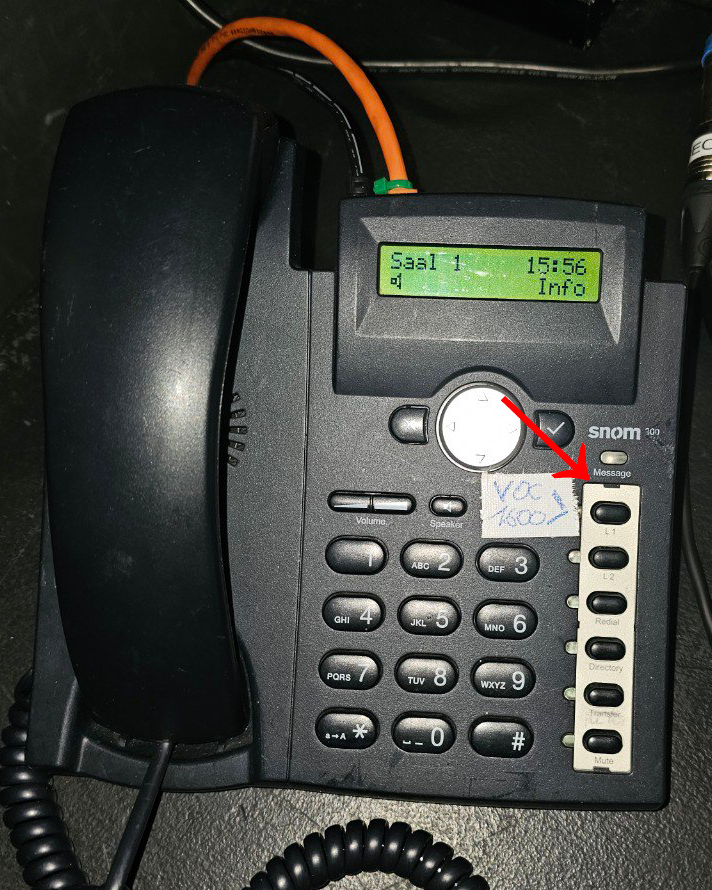
\includegraphics[width=0.5\textwidth]{images/telephone.png}
			\caption{Telephone on Mixer Desk}
		\end{figure}
		\column{0.5\textwidth}
		\begin{itemize}
		\item If there are any issues, contact us via Telephone. Just press the VOC Button (red arrow)
		\item Call us via DECT 1600 and state the lecture hall you are in.
		\end{itemize}
		
	\end{columns}
\end{frame}

%\begin{frame}{Radio}
%	\begin{columns}[T,onlytextwidth]
%		\column{0.5\textwidth}
%		\begin{figure} 
%			\centering
%			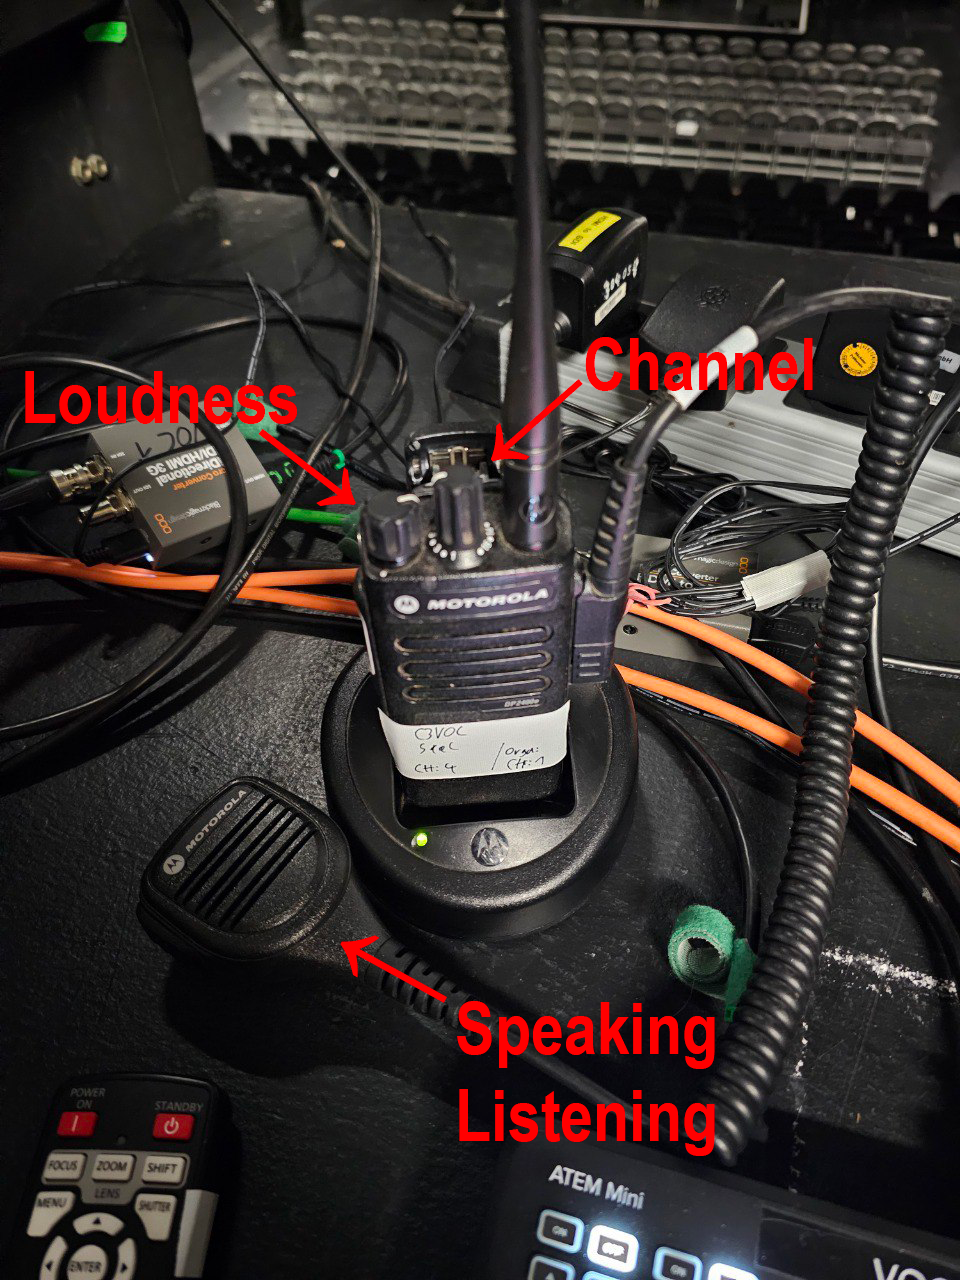
\includegraphics[width=0.65\textwidth]{images/radio.png}
%			\caption{C3ROC Radio Device}
%		\end{figure}
%		\column{0.5\textwidth}
%		Radios are used for communicating and fixing issues. 
%		You can clip the device on, but please put it back in the charger after your shift. 
%		\begin{description}
%			\item[Channel] Ensure that the device is set on \textbf{ channel 4 }
%			\item[Volume] Check loudspeaker volume by switching to a different channel and back. Should be loud enough to hear, but not too loud to annoy the audience.
%		\end{description}
%	\end{columns}
%\end{frame}

%\begin{frame}{Radio Discipline}
%	\begin{columns}[T,onlytextwidth]
%		\column{0.3\textwidth}
%		\begin{figure} 
%			\centering
%			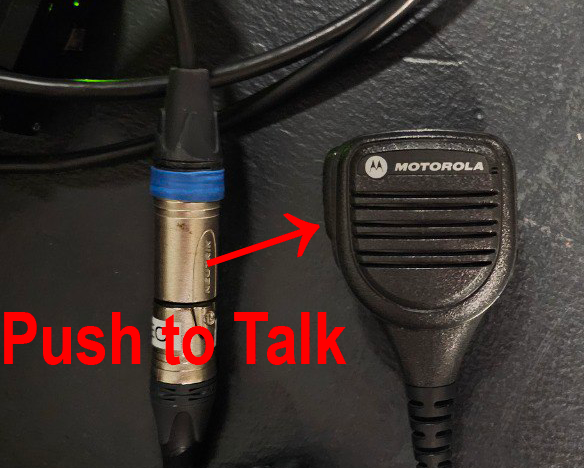
\includegraphics[width=0.75\textwidth]{images/radio_ptt.png}
%			\caption{PTT}
%		\end{figure}
%		\column{0.7\textwidth}
%		One way communication only, either speak or listen. The device takes some time to connect.
%		\begin{description}
%			\item[Think] Prior pressing the button, think about what you want to say.
%			\item[Press] Press the button, but don't start speaking immediately.
%			\item[Wait] Ready state signalled by a short beep.
 %           \item[Hail] Start with C3VOC followed by your name
%			\item[Speak] Tell us about your issue and release the button.
%            \item[Listen] Listen to any answers.
%		\end{description}
%		\end{columns}
%\end{frame}

%\begin{frame}{Intercom: Mixer }
%	\begin{columns}[T,onlytextwidth]
%		\column{0.5\textwidth}
%		\begin{figure} 
%			\centering
%			\includegraphics[width=0.9\textwidth]{images/intercom-Mixer.png}
%			\caption{Intercom Device: Main Station}
%		\end{figure}
%		\column{0.5\textwidth}
%			We use an Party-Line intercom for communication between mixer and camera
%"		\begin{description}
%			\item[Headset VOL] Adjust the loudness of your headset
%			\item[PPT] PPT Should switched to "off", so you can always speak to the camera angel
%		\end{description}
%	\end{columns}
%\end{frame}

%\begin{frame}{Intercom: Camera }
%	\begin{columns}[T,onlytextwidth]
%		\column{0.5\textwidth}
%		\begin{figure} 
%			\centering
%			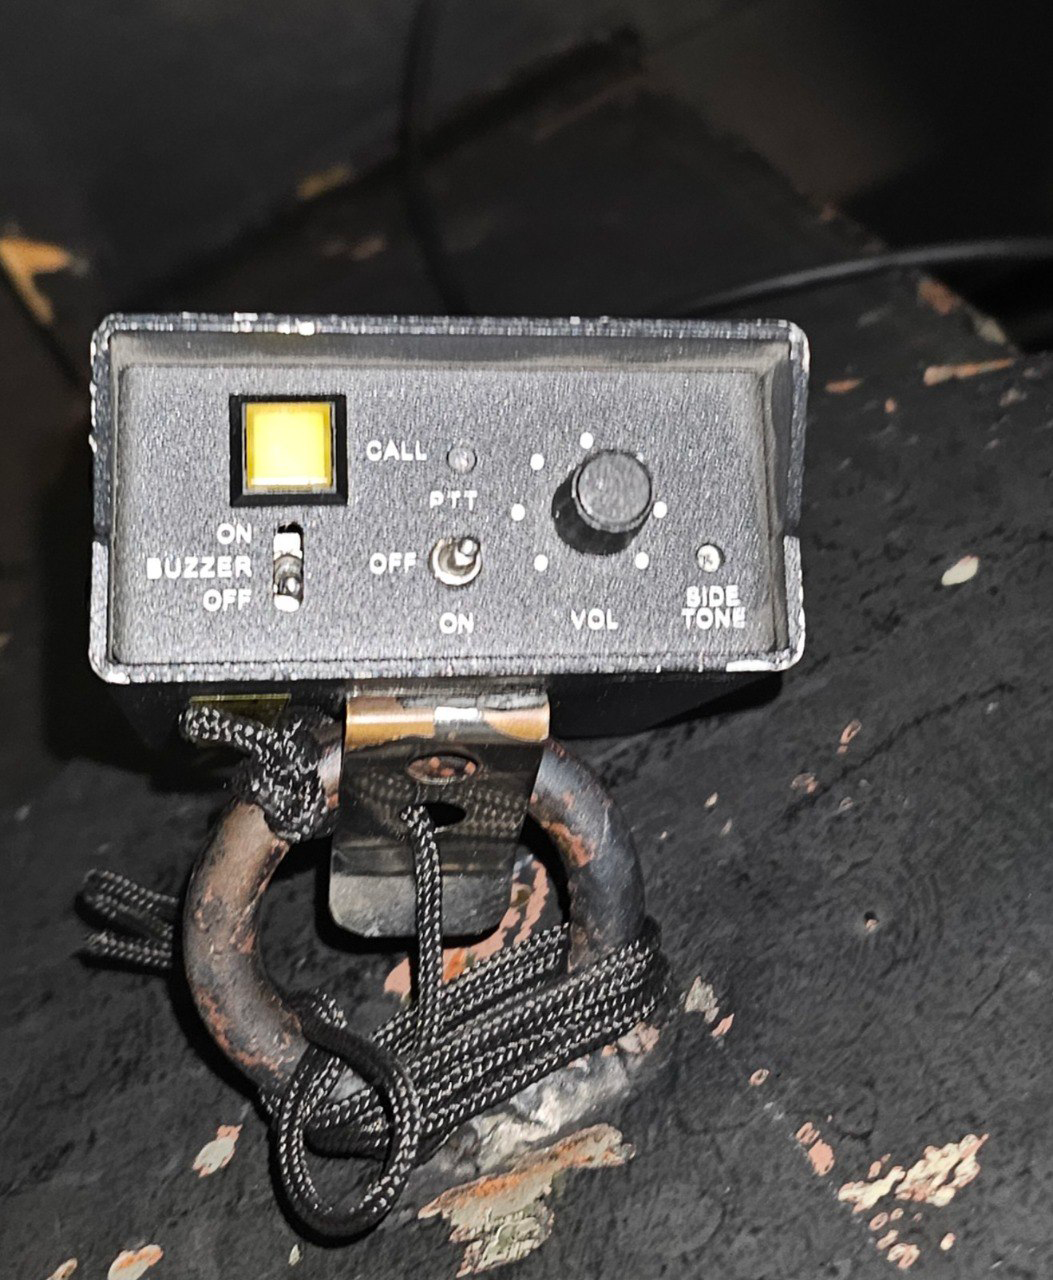
\includegraphics[width=0.75\textwidth]{images/intercom-camera.png}
%			\caption{Intercom Device: Camera Station}
%		\end{figure}
%		\column{0.5\textwidth}
%
%		\begin{description}
%			\item[VOL] Adjust volume prior talk.
%			\item[PTT] Ensure that PTT is set to "off", to prevent noise from the stage on the party line.
%			\item[Yellow Button] Press the yellow button to speak.
%		\end{description}
%	\end{columns}
%\end{frame}
